\documentclass{report}

\usepackage[ngerman]{babel}
\usepackage[utf8]{inputenc}
\usepackage[T1]{fontenc}
\usepackage{hyperref}
\usepackage{csquotes}
\usepackage[a4paper]{geometry}
\usepackage{graphicx}

\usepackage[
    backend=biber,
    style=apa,
    sortlocale=de_DE,
    natbib=true,
    url=false,
    doi=false,
    sortcites=true,
    sorting=nyt,
    isbn=false,
    hyperref=true,
    backref=false,
    giveninits=false,
    eprint=false]{biblatex}
\addbibresource{../references/bibliography.bib}


\title{Ethik im Umgang mit Daten}
\author{D'Ambrosio Pietro}
\date{\today}


\begin{document}

\maketitle

\abstract{
In diesem Dokument habe ich mich mit KI, Bias und mit der Frage 
beschäftigt:Was sind die Risiken von Bias in KI-Systemen und wie kann man diese minimieren?}

\tableofcontents
\newpage
\chapter{Einleitung}
Eine Perfekte Einleitung ins Thema wäre eine von ChatGPT generierte 
zusammenfassung über Daten, Ethik und KI zum zeigen wie hilfreich dieses Tool ist.
"Künstliche Intelligenz (KI) verwendet Daten, um anhand von Mustern zu 
erlernen und Entscheidungen zu treffen. Dadurch ist KI in vielen Bereichen 
ein mächtiges Instrument. Die Ethik im Bereich der KI behandelt die moralischen 
Fragen und Schwierigkeiten, die sich aus der Anwendung dieser Technologien ergeben, 
vor allem in Bezug auf Fairness, Transparenz und Rechenschaftspflicht. Die Verbindung 
zwischen KI, Daten und Ethik besteht darin, wie Daten gesammelt, genutzt und verarbeitet 
werden, um die faire und unvoreingenommene Entscheidungsfindung von KI-Systemen zu gewährleisten. 
Im Verlauf des Dokuments wird jedoch erläutert, warum dies unmöglich ist. Um sicherzustellen, 
dass KI-Systeme die Rechte und Würde aller Menschen achten, sind ethische Grundsätze von entscheidender 
Bedeutung."



\input{KI_einführung.tex}
\chapter{Kognitive Verzerrung/Bias}
In diesem Kapitel bearbeite ich meine Hauptfrage: 
Was sind die Risiken von Bias in KI-Systemen und wie kann man diese minimieren?
      
     
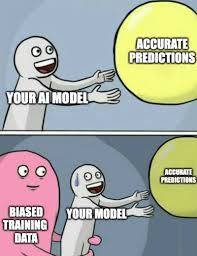
\includegraphics[width=0.25\textwidth]{images.jpg}
\input{Bias_einführung.tex}

\section{Was sind Ursachen von Bias?}
Einige Ursachen von Bias sind die Beurteilung des Aussehens von Menschen, 
vorgefasste Meinungen, logische Fehlschlüsse und die Entscheidungsfindung basierend
auf Emotionen. Diese können entstehen von Ereignisse von der Vergangenheit, fehlinformationen
von Social Media oder allgemeine fehlende Fähigkeiten Personen richtig einzuschätzen.
Aufgelistet sind Hier die häufigsten Voreingenommenheiten.
\begin{itemize}
    \item Geschlechtsbezogene Vorurteile
    \item Altersdisskriminierung
    \item Voreingenommenheit auf Grund des Namens
    \item Voreingenommenheit auf Grund der Attraktivität
    \item Voreingenommenheit durch Selbstüberschätzung
    \item Wahrnehmungsfehler
    \item Voreingenommenheit auf Grund des Aussehens
\end{itemize} \citep{Ursachen_Bias}
\section{Was sind die Folgen von Bias?}
Ein BEispiel hierführ wäre das Ereigniss aus 2019 in den USA.
In den Vereinigten Staaten wurde eine KI eingesetzt, um die 
Gesundheitsversorgung so effektiv wie möglich zu gestalten. 
Diese dient dazu, Patienten*innen mit speziellem Pflegebedarf zu 
identifizieren. 
Eine Studie, die im Oktober 2019 veröffentlicht wurde, weist jedoch darauf hin, 
dass Afroamerikaner*innen mit derselben Schwere der Erkrankung weniger 
häufig als Weiße für eine zusätzliche Pflege vorgeschlagen worden sind. 
Eine KI ohne Zweifel hätte in der Tat die doppelte Anzahl von Afroamerikaner*innen mit 
speziellem Pflegebedarf erfassen sollen. Wie ist eine KI, die eigentlich 
„farbenblind“ ist, zu diesen Resultaten gelangt?
Das Risiko der Patient*innen wurde durch den Algorithmus 
dieser KI als die voraussichtlichen Ausgaben für eine weitere Behandlung
festgelegt. Da der US-amerikanische Staat aufgrund verschiedener Faktoren weniger Geld für die 
Behandlung von Afroamerikaner*innen ausgibt, wurden die Ausgaben und damit auch das 
Risiko für Personen dieser ethnischen Gruppe als niedriger bewertet.
\citep{Folgen_Bias}
\input{Bias_lösungen.tex}
\newpage
\chapter{Fazit}
In diesem Kapitel habe ich meine Fazit über, was sind die Risiken von Bias in KI-Systemen
und wie kann man diese minimieren.

\vspace{5mm}Kognitive Verzerrungen sind Voreingenommenheiten oder Abweichungen von klaren 
Standards im menschlichen Verhalten. Diese Verzerrungen beeinflussen 
auch Künstliche Intelligenz (KI), die auf voreingenommenen Daten basieren
kann und somit beispielsweise zu diskriminierenden Entscheidungen führen kann.
Ursachen von Bias umfassen vorgefasste Meinungen, emotionale 
Entscheidungen und historische Ereignisse. Diese Verzerrungen 
betreffen verschiedene Bereiche wie Geschlecht, Alter und Aussehen.
Die Folgen von Bias sind gravierend, wie das Beispiel der 
Gesundheitsversorgung in den USA zeigt, wo Afroamerikaner*innen benachteiligt wurden.
Um Bias in KI zu reduzieren, sollten verschiedene Datenquellen genutzt, 
transparente Algorithmen entwickelt, Ethikrichtlinien implementiert
und Bias-Training durchgeführt werden. Diese Maßnahmen würden jegliche KI sehr fördern 
und es würden mehr faire und ausgewogene KI-Systeme geben die auch in der Gesellschaft besser genutzt werden
können.

\printbibliography

\end{document}
